
\chapter{Dos Resultados Obtidos}
\label{cap:results}
\minitoc

\intro{Neste capítulo serão mostrados os resultados deste trabalho. Mas como fazer isso se capturas de tela
não são capazes de mostrar a aplicação funcionando ao vivo? A ideia é ilustrar as funcionalidades principais
enquanto o link da aplicação em produção ficará diponível aqui.

Outro ponto importante a mostrar aqui é a cobertura de testes. A cobertura do frot não será tão extensiva
quanto a do back, mas ao comparar com o que se tinha no começo do ano, é infinitamente maior. }

\section{O que foi feito?}
\label{sec:to-be-done}

Na sessão \ref{sec:goals} fala-se que um dos objetivos era fazer um sistema eficiente com código limpo. Esse sistema
divide-se em dois: a API feita em Rails e a interface de usuário feita em Nuxt.

\subsection{API Rails}\label{subsec:api-rails}

Nessa parte, o principal feito foi uma grande refatoração. Muita coisa precisava ser refatorada e 90\% do tempo dedicado
a este trabalho envolveu a refatoração do que tinha sido feito ano passado. O motivo não era um mal funcionamento, ou
uma lógica equivocada. O código funcionava muito bem, mas estava engessado, e sem testes. Tudo foi devidamente acertado.
Para ver as rotas criadas, vale ver o arquivo \texttt{delpo/config/routes}

\begin{figure}[h]
  \centering
  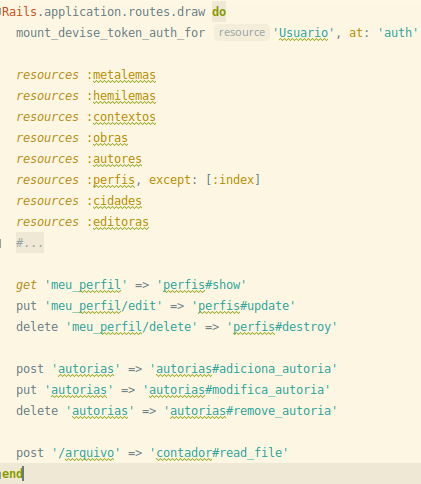
\includegraphics[width=.6\textwidth]{figuras/rails_routes.png}
  \caption{Arquivo de rotas}
  \label{fig:routes_files}
\end{figure}

Observações sobre a figura:
\begin{itemize}
  \item \texttt{mount\_devise\_token\_auth\_for} é um comando que gera as rotas para os controladores do Devise
  \item \texttt{resources} é a palavra chave que gera as rotas de CRUD (Create/Read/Update/Delete) para um determinado
  recurso
\end{itemize}

Na figura \ref{fig:mvc}, vimos como uma aplicação MVC funciona. Entretanto, como não há visualização na aplicação em Rails,
a gema \texttt{Active Model Serializer} substituiu o sistema que produz o conteúdo a partir de arquivos \texttt{.html.erb}.
Para mostrar algumas rotas funcionando, usarei um cliente HTTP chamado Insomnia\footnote{Vale saber que, ao usar esse
programa, há abas específicas para se colocar os cabeçalhos das requisições. A única motivação para colocá-los junto aos
dados enviados é capturar esses detalhes em uma única captura}. Os valores descritos nas capturas de tela são ilustrativos.

\subsubsection{Cadastro}

\begin{figure}[ht]
  \centering
  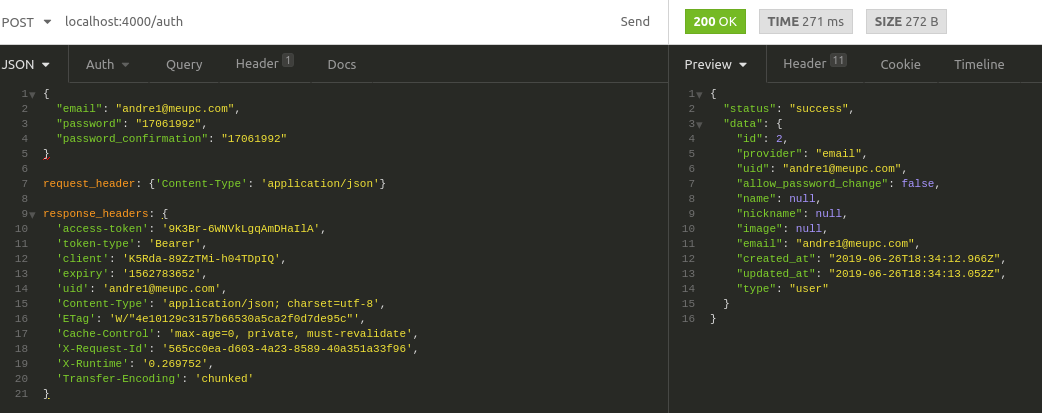
\includegraphics[width=.75\textwidth]{figuras/sign-up.png}
  \caption{\texttt{POST /auth}}
  \label{fig:sign-up}
\end{figure}

Na figura acima, como podemos ver como o cadastro de novos pesquisadores é feito pelo backend. Os dados retornados são
o status da requisição como uma representação em JSON do objeto \texttt{Usuario}. Os cabeçalhos da resposta permitem que
o usuário possa ser reconhecido, e portanto, autenticado (especificamente os campos \texttt{uid}, \texttt{client} e
\texttt{access-token}). Não é necessário fazer login depois de se cadastrar. Pode apresentar falhas se o usuário utilizar
um email repetido, ou se os cabeçalhos estiverem incorretos.

\subsubsection{Log-in}

\begin{figure}[ht]
  \centering
  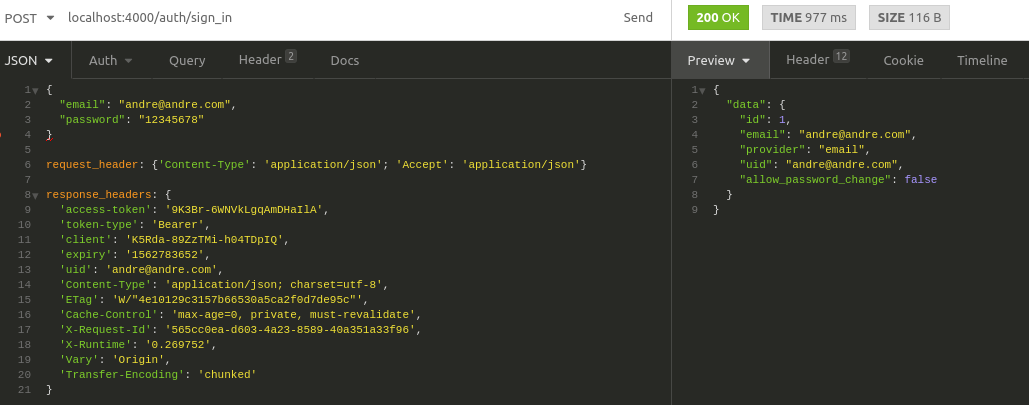
\includegraphics[width=.75\textwidth]{figuras/sign-in.png}
  \caption{\texttt{POST /auth/sign\_in}}
  \label{fig:sign-in}
\end{figure}

Muito similar ao controlador anterior, e retorna praticamente as mesmas coisas que a requisição anterior. Da mesma forma
que a requisição acima, providencia dados suficientes para que o usuário seja reconhecido pelo sistema. Ao contrário do
processo de cadastro, destina-se a quem já tem um usuário cadastrado no sistema. Pode falhar se não houver usuário
cadastrado com os dados fornecidos.

\subsubsection{Criando Perfis}

\begin{figure}[h]
  \centering
  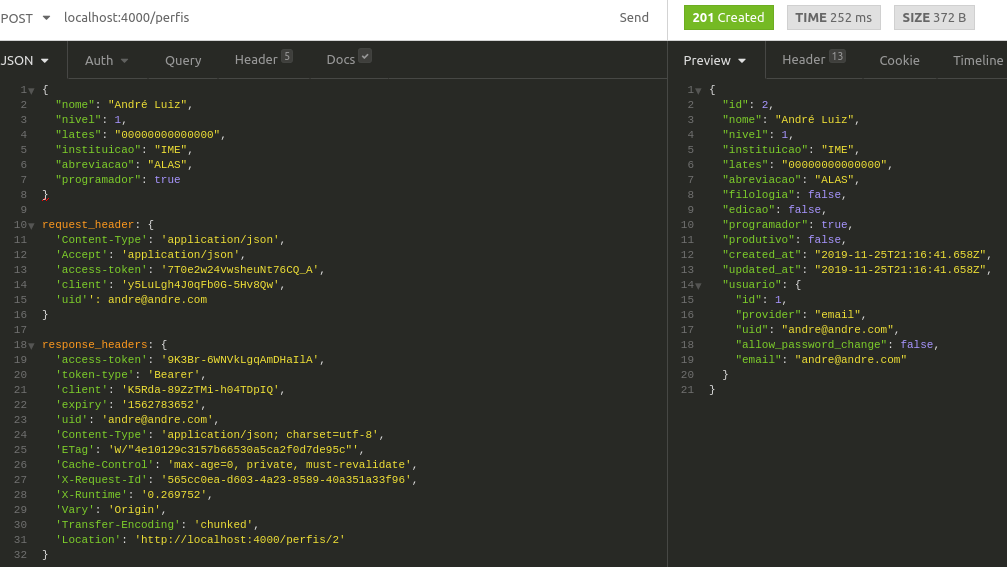
\includegraphics[width=.75\textwidth]{figuras/novo-perfil.png}
  \caption{\texttt{POST /perfis}}
  \label{fig:novo-perfil}
\end{figure}

Depois de se logar, é necessário criar um perfil para usar os recursos mais avançados do portal. Para fazer isso, é
necessário ter um usuário logado. Esse usuário, identificado por campos já mencionados, será associado ao perfil a ser
criado. Os campos necessários na requisição para criação do perfil são:
\begin{itemize}
  \item nome
  \item lates
  \item abreviação
  \item instituição
  \item tipo de pesquisador (filologia, edição, programador, produtivo)
\end{itemize}

No primeiro momento, os cabeçalhos da resposta vão retonar valores praticamente constantes, entretanto, e por motivos de
segurança, é recomendável modificar os tokens de acesso a cada nova requisição. Isso está na lista de coisas a implementar.

\subsubsection{Vendo um perfil \hfill figura \ref{fig:ver-perfil}}

\begin{figure}[ht]
  \centering
  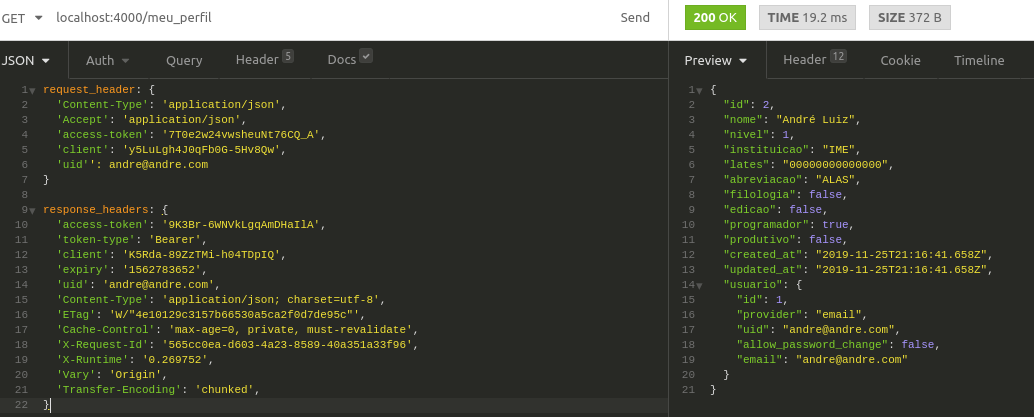
\includegraphics[width=.75\textwidth]{figuras/ver-perfil.png}
  \caption{\texttt{GET /meu\_perfil} ou \texttt{GET /perfis/:id}}
  \label{fig:ver-perfil}
\end{figure}

A única coisa que é necessário para realizar essa requisição é ter um usuário autenticado (usando os campos de cabeçalho
já mencionados) e um identificador de usuário. As requisições retornam os dados do perfil do usuário em questão ou de
algum perfil específico. Vai dar erro se não houver um usuário autenticado.

\subsubsection{Log-off \hfill figura \ref{fig:saindo}}

\begin{figure}[ht]
  \centering
  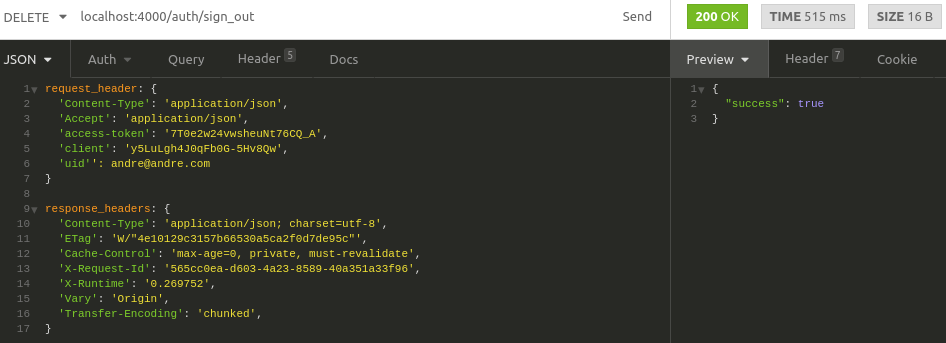
\includegraphics[width=.75\textwidth]{figuras/sign-out.png}
  \caption{\texttt{DELETE /sign\_out}}
  \label{fig:saindo}
\end{figure}

A requisição usada para sair do perfil/sessão. Precisa apenas de alguém logado, e não retorna dados muito relevantes.

\subsection{Interface de usuário}\label{subsec:gui}

A interface do usuário foi a última parte a ser desenvolvida, e ficou incompleta. Entretanto, já conta com todos os
conteúdos estáticos do site original, e as mesmas cores básicas\footnote{Graças a um programa que detecta especificamente
que cor está no espaço apontado chamado \href{http://www.gpick.org/}{Gpick}}. Além disso, o sistema de log-in está
concluído e funcionando, sendo esse meu ponto de parada antes da entrega. Abaixo encontram-se duas capturas de telas para
ilustrar como está a página atualmente

\begin{figure}[htb]
  \centering
  \subfloat[\texttt{/home}]{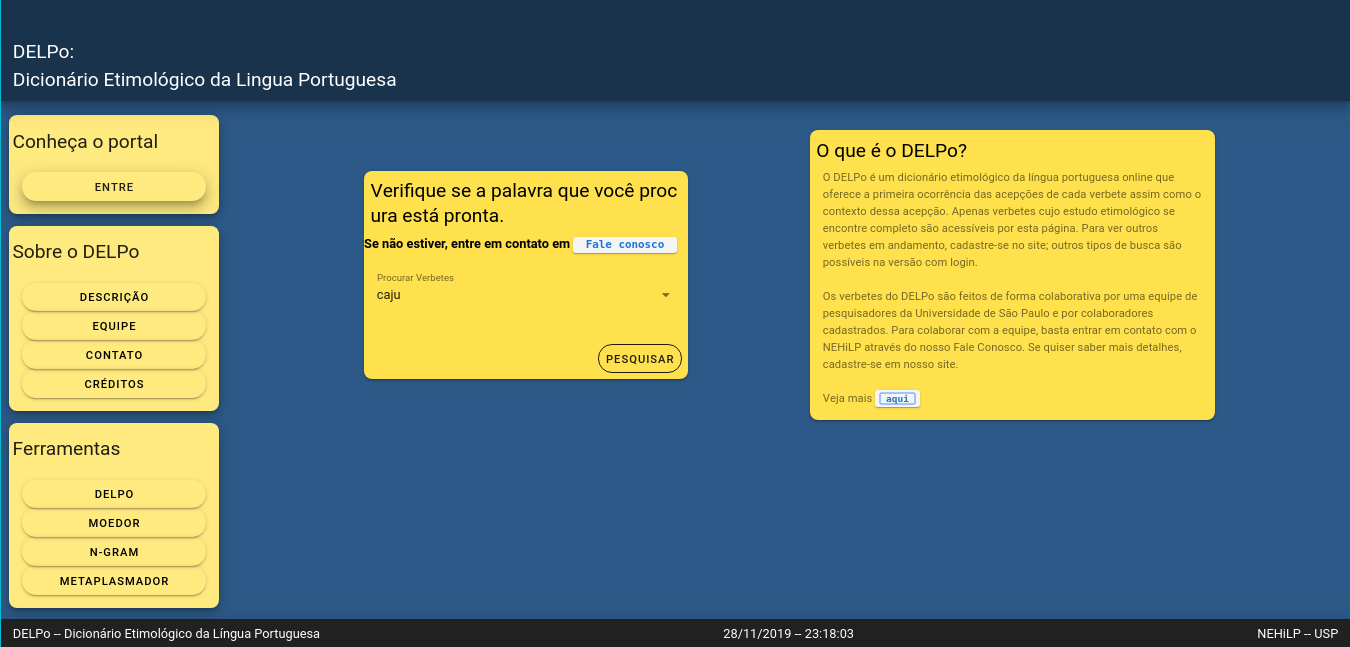
\includegraphics[width=.5\textwidth]{figuras/home.png}}
  \subfloat[\texttt{/equipe}]{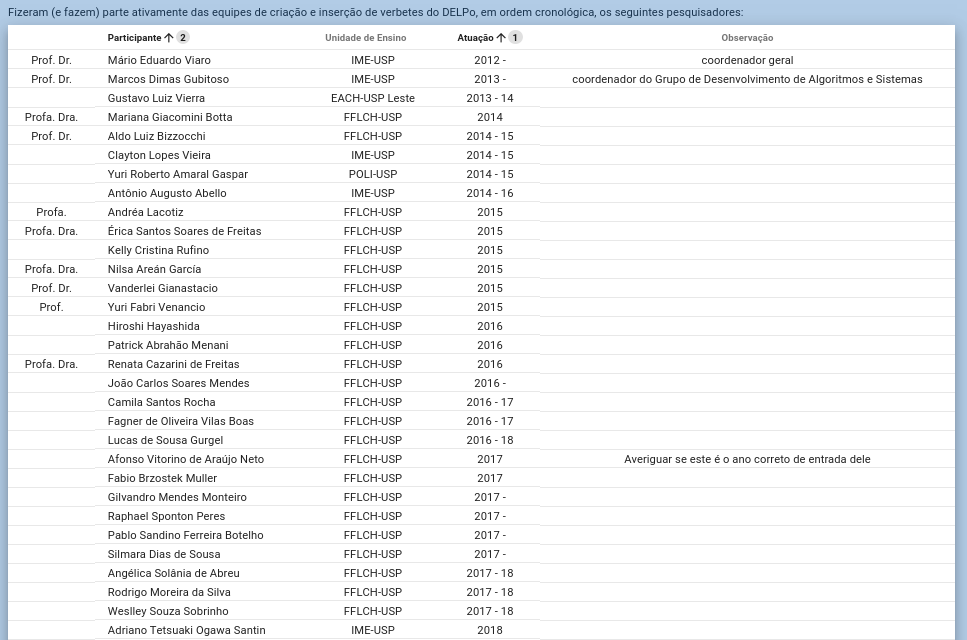
\includegraphics[width=.35\textwidth]{figuras/lista_pesquisadores.png}}
  \caption{Captura de telas feitas a partir da interface}
  \label{fig:screenshots}
\end{figure}

\subsection{O moedor}\label{subsec:o-moedor}

Como foi dito na sessão \ref{sec:proposta}, o moedor é um punhado gigantesco de código com uma necessidade enorme de
ser refatorado. Não porque é ruim ou está incorreto, mas por estar extremamente confuso, com as responsabilidades
misturadas, funções enormes\footnote{Sendo a maior a \texttt{processa\_contextos} com exatas 962 linhas à época da
contagem}. A função \texttt{initialize} também precisam de modificações, mas fica para a list de refatorações a fazer.

A ideia é mover para os \emph{helpers} tudo exceto pela função de inicialização e de leitura. O que for para os helpers,
será testado.

\subsection{Testes e cobertura}
\label{subsec:testes-cobertura}

Uma das propostas do projeto era ter uma cobertura razoável de testes. Na aplicação Rails isso foi feito de fato. No
aplicação Nuxt, entretanto, não foi possível\footnote{Motivo espresso na sessão \ref{subsec:no-tests-for-nuxt}}. Tendo
dito, aqui está um print que comprova a cobertura de testes no back end no momento da entrega de monografia. Este
relatório é produzido por uma gema chamada \texttt{simple-cov}. Ao executar os testes, o sistema entra em ação e gera um
painel que permite ao desenvolvedor saber que módulos ou classes precisam de mais cobertura.

\begin{figure}[htb]
  \centering
  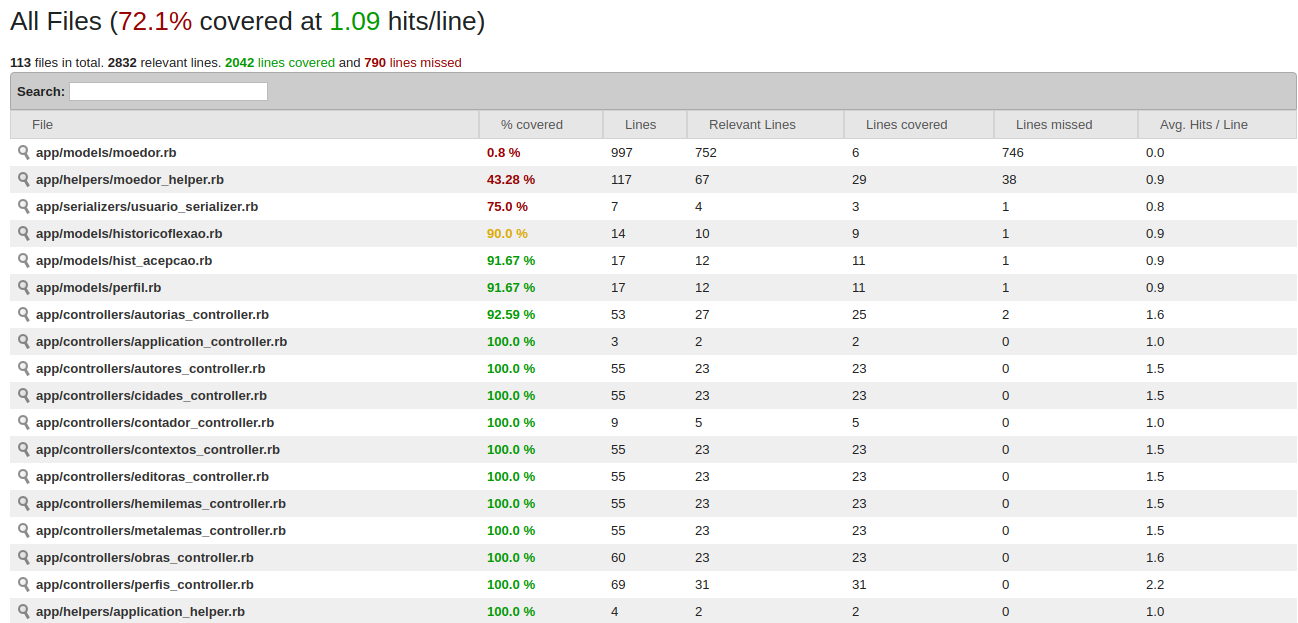
\includegraphics[width=.9\textwidth]{figuras/test_coverage.png}
  \caption{Parte do relatório de cobertura de testes}
  \label{fig:test-coverage}
\end{figure}

\section{O que será feito?}
\label{sec:what-will-be-done}

Mesmo depois de concluído a disciplina, pretendo ainda contribuir para o projeto, e isso abre oportunidades de implementar
mais coisas, além de terminar o que foi iniciado, claro.

\subsection{Atividades Em Andamento}\label{subsec:ongoing}

Segue um detalhamento sobre os detalhes que faltam para completar certos os pontos levantados na tabela \ref{table:activity}

\subsubsection{Fazer uma interface de usuário agradável}

\begin{itemize}
  \item Completo o sistema de login, é necessério inserir a funcionalidade de moagem e estudar como serão mostrados os
  resultados
  \item Falta criar um painel de controle do usuário onde ele possa interagir com as atividades que ele pode usar, e fazer
  suas pesquisas --- isso pode depender da implementação de controladores que antes não eram necessários
\end{itemize}

\subsubsection{Fazer os testes da aplicação Rails}

\begin{itemize}
  \item Depende de continuar refatorando código antigo
  \item Como ficou claro na figura \ref{fig:test-coverage}, os arquivos com menos (abaixo de 90\%) cobertura foram
  \begin{itemize}
    \item \texttt{app/models/moedor.rb}
    \item \texttt{app/helpers/moedor\_helper.rb}
  \end{itemize}
  \item No caso desses aquivos, o problema é a quantidade de métodos ainda sem refatoração.
\end{itemize}

\subsubsection{Refatorar o moedor}

O que falta pra concluir essa tarefa é quebrar dois métodos que dependem de consultas em SQL utilizando o
\emph{ActiveRecord}. Outra coisa importantíssima e potencialmente desafiadora é quebrar o método
\texttt{processa\_contextos} que conta com 962 linhas. O \texttt{initialize}  dessa classe (que pode ser engolida pelo
método de mesmo nome) também deve ser quebrado em alguns outros.

\subsection{Atividades A Fazer}\label{subsec:to-do}

\paragraph{Adaptação do conteúdo do outro banco de dados} Pode não ser o maior dos desafios, mas pode dar bastante
trabalho. Trata-se de colocar os dados do banco de dados da aplicação atualmente em produção, e passá-los para a
aplicação Rails.

\paragraph{Fazer os testes do front} A ideia para testar a aplicação em Nuxt é assistir um curso da plataforma
\href{https://vueschool.io/}{\textbf{Vue School}} voltado a como testar componentes Vue com Jest. O propósito é usar meus
componentes como material de exercício dessas aulas. Depois de testar o que foi feito até agora, posso começar a
implementar com base em componentes que ainda pretendo implementar

\subsection{Refatorações}\label{subsec:refatoracoes}

Além da refatoração do moedor já mencionada, é possível que se implemente um construtor de formulários e botões. Tudo
para repetir menos código e facilitar os testes.
